\chapter{Components Sim\`{e}triques} \index{components sim\`{e}triques}

La teoria de les components sim\`{e}triques \'{e}s \'{u}til en l'estudi de
tensions i corrents trif\`{a}sics
 desequilibrats, com ara els que es produeixen en un curt circuit on no intervenen les tres
 fases a l'hora (curt circuit fase--terra, fase--fase, etc.).

\section{L'operador complex {"<}a{">}}

Definim en primer lloc l'operador complex {"<}a{">}, el qual t\'{e} un m\`{o}dul
igual a la unitat i un argument igual a $120\degree$: \index{a}
\begin{equation}
   \au \equiv 1_{\measuredangle 120\degree} = \eu^{\ju\frac{2\piup}{3}} =
   \cos \frac{2\piup}{3} + \ju \sin \frac{2\piup}{3} = - \frac{1}{2} + \ju \frac{\sqrt{3}}{2}
\end{equation}

A l'hora d'operar amb aquest valor, resulten \'{u}tils les relacions
seg\"{u}ents:
\begin{equation}
   \au^2 = 1_{\measuredangle 240\degree}= - \frac{1}{2} - \ju \frac{\sqrt{3}}{2}\qquad\qquad
   \au^3 = 1_{\measuredangle 0\degree} \qquad\qquad
   1+ \au + \au^2 = 0
\end{equation}

\section{\texorpdfstring{Teorema de Fortescue--Stokvis}{Teorema de Fortescue-Stokvis}}\index{teorema!de Fortescue--Stokvis}

Tal com es veu en la Figura \vref{pic:Comp_sim}, aquest teorema
estableix que qualsevol sistema trif\`{a}sic asim\`{e}tric (tamb\'{e} anomenat
desequilibrat),  es pot descompondre  en la suma de tres sistemes
sim\`{e}trics: un sistema directe o de seq\"{u}\`{e}ncia positiva, un sistema
invers o de seq\"{u}\`{e}ncia negativa, i un sistema homopolar o de
seq\"{u}\`{e}ncia zero. Els vectors $\cmplx{\chi}_\alphaup$,
$\cmplx{\chi}_\betaup$ i $\cmplx{\chi}_\gammaup$, poden representar tant
tensions com corrents.
\begin{figure}[h]
\centering
    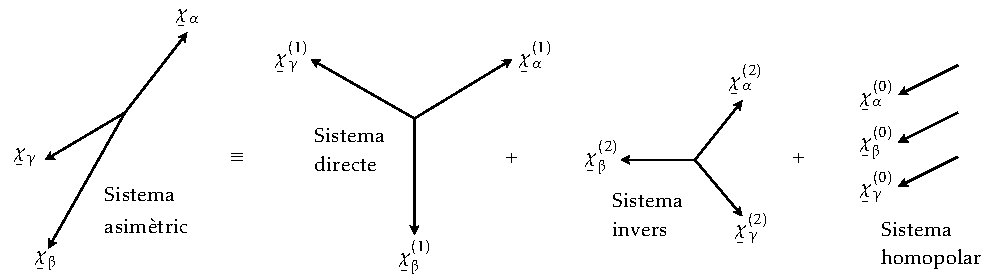
\includegraphics{Imatges/Cap-CompSim-CompSim.pdf}
\caption{Components sim\`{e}triques. Teorema de Fortescue--Stokvis}
\label{pic:Comp_sim}
\end{figure}

\index{sistema!directe} \index{sistema!invers}
\index{sistema!homopolar} El sistema directe est\`{a} format per tres
vectors que tenen la mateixa seq\"{u}\`{e}ncia de fases que els vectors
originals, per exemple: $\alphaup$-$\betaup$-$\gammaup$; els vectors
s'identifiquen mitjan\c{c}ant els super\'{\i}ndexs {"<}(1){">} o {"<}(d){">}. El sistema
invers est\`{a} format per tres vectors que tenen la seq\"{u}\`{e}ncia contr\`{a}ria
de fases que els vectors originals, per exemple:
$\alphaup$-$\gammaup$-$\betaup$; els vectors s'identifiquen mitjan\c{c}ant els
super\'{\i}ndexs {"<}(2){">} o {"<}(i){">}. Finalment, el sistema homopolar est\`{a}
format per tres vectors que estan en fase entre si; els vectors
s'identifiquen mitjan\c{c}ant el super\'{\i}ndex {"<}(0){">}.

Per tant, expressant els vectors del sistema asim\`{e}tric en funci\'{o}
dels vectors dels tres sistemes sim\`{e}trics, tenim:
\begin{subequations}
\begin{align}
   \cmplx{\chi}_\alphaup &= \cmplx{\chi}_\alphaup\ap{(0)}  +
   \cmplx{\chi}_\alphaup\ap{(1)} + \cmplx{\chi}_\alphaup\ap{(2)} \label{eq:c_sim_a}\\
   \cmplx{\chi}_\betaup &= \cmplx{\chi}_\betaup\ap{(0)} + \cmplx{\chi}_\betaup\ap{(1)} +
   \cmplx{\chi}_\betaup\ap{(2)}  =  \cmplx{\chi}_\alphaup\ap{(0)} + \au^2
   \cmplx{\chi}_\alphaup\ap{(1)} + \au \cmplx{\chi}_\alphaup\ap{(2)} \label{eq:c_sim_b}\\
   \cmplx{\chi}_\gammaup &= \cmplx{\chi}_\gammaup\ap{(0)} + \cmplx{\chi}_\gammaup\ap{(1)} +
   \cmplx{\chi}_\gammaup\ap{(2)}  = \cmplx{\chi}_\alphaup\ap{(0)} + \au
   \cmplx{\chi}_\alphaup\ap{(1)} + \au^2 \cmplx{\chi}_\alphaup\ap{(2)} \label{eq:c_sim_c}
\end{align}
\end{subequations}

o en forma matricial:
\begin{equation}
   \begin{pmatrix}
     \cmplx{\chi}_\alphaup \\
     \cmplx{\chi}_\betaup \\
     \cmplx{\chi}_\gammaup
   \end{pmatrix} =
   \begin{pmatrix}
     1 & 1 & 1 \\
     1 & \au^2 & \au\\
     1 & \au & \au^2
   \end{pmatrix} \cdot
   \begin{pmatrix}
     \cmplx{\chi}_\alphaup\ap{(0)} \\
     \cmplx{\chi}_\alphaup\ap{(1)} \\
     \cmplx{\chi}_\alphaup\ap{(2)}
   \end{pmatrix}
\end{equation}

A partir del sistema d'equacions anterior, podem trobar els vectors
dels tres sistemes sim\`{e}trics en funci\'{o} dels vectors del sistema
asim\`{e}tric:
\begin{subequations}
\begin{align}
   \cmplx{\chi}_\alphaup\ap{(0)} &= \frac{1}{3} (\cmplx{\chi}_\alphaup + \cmplx{\chi}_\betaup +
   \cmplx{\chi}_\gammaup) & \cmplx{\chi}_\betaup\ap{(0)} &= \cmplx{\chi}_\alphaup\ap{(0)} &
   \cmplx{\chi}_\gammaup\ap{(0)} &= \cmplx{\chi}_\alphaup\ap{(0)}
   \label{eq:c_sim_c2}\\
   \cmplx{\chi}_\alphaup\ap{(1)} &= \frac{1}{3} (\cmplx{\chi}_\alphaup + \au \cmplx{\chi}_\betaup +
   \au^2 \cmplx{\chi}_\gammaup) & \cmplx{\chi}_\betaup\ap{(1)} &= \au^2 \cmplx{\chi}_\alphaup\ap{(1)} &
   \cmplx{\chi}_\gammaup\ap{(1)} &= \au \cmplx{\chi}_\alphaup\ap{(1)} \label{eq:c_sim_a2} \\
   \cmplx{\chi}_\alphaup\ap{(2)} &= \frac{1}{3} (\cmplx{\chi}_\alphaup + \au^2 \cmplx{\chi}_\betaup +
   \au \cmplx{\chi}_\gammaup) & \cmplx{\chi}_\betaup\ap{(2)} &= \au \cmplx{\chi}_\alphaup\ap{(2)} &
   \cmplx{\chi}_\gammaup\ap{(2)} &= \au^2 \cmplx{\chi}_\alphaup\ap{(2)} \label{eq:c_sim_b2}
\end{align}
\end{subequations}

o en forma matricial:
\begin{equation}
   \begin{pmatrix}
     \cmplx{\chi}_\alphaup\ap{(0)} \\
     \cmplx{\chi}_\alphaup\ap{(1)} \\
     \cmplx{\chi}_\alphaup\ap{(2)}
   \end{pmatrix} =
   \begin{pmatrix}
     1 & 1 & 1 \\
     1 & \au^2 & \au\\
     1 & \au & \au^2
   \end{pmatrix}^{-1} \cdot
   \begin{pmatrix}
     \cmplx{\chi}_\alphaup \\
     \cmplx{\chi}_\betaup \\
     \cmplx{\chi}_\gammaup
   \end{pmatrix} =  \frac{1}{3} \cdot
   \begin{pmatrix}
     1 & 1 & 1 \\
     1 & \au & \au^2 \\
     1 & \au^2 & \au
   \end{pmatrix} \cdot
   \begin{pmatrix}
     \cmplx{\chi}_\alphaup \\
     \cmplx{\chi}_\betaup \\
     \cmplx{\chi}_\gammaup
   \end{pmatrix}
\end{equation}

\section{Corrent de neutre} \index{corrent de neutre}

Suposem un sistema trif\`{a}sic amb neutre de retorn, que pot ser el
terra, on qualsevol de les seves parts (generador, l\'{\i}nia o consum)
poden ser desequilibrades; el corrent que circula pel neutre \'{e}s
sempre la suma dels tres corrents de fase: $\cmplx{I}_\alphaup+
\cmplx{I}_\betaup+\cmplx{I}_\gammaup$. A partir d'aquest fet, i
observant l'equaci\'{o} \eqref{eq:c_sim_c2}, es veu que el corrent de
retorn pel neutre, \'{e}s igual a tres vegades la component homopolar
del sistema de corrents de fase:
\begin{equation}
    \cmplx{I}_\alphaup+\cmplx{I}_\betaup+\cmplx{I}_\gammaup =3 \cmplx{I}_\alphaup\ap{(0)}
\end{equation}

D'altra banda, quan un sistema trif\`{a}sic no t\'{e} neutre, tenim
$\cmplx{I}_\alphaup+ \cmplx{I}_\betaup+\cmplx{I}_\gammaup=0$, i per tant,
observant la mateixa equaci\'{o} \eqref{eq:c_sim_c2}, es veu que el
sistema format pels corrents de fase no t\'{e} sistema homopolar.

Finalment, tamb\'{e} podem dir que el corrent total a terra, en cas de
defecte a terra, \'{e}s igual a tres vegades la component homopolar del
corrent de curt circuit.

\section{Propietats de les tensions fase--fase i fase--neutre}\label{sec:comp-sim-neutre}
\index{tensi\'{o}!fase--fase} \index{tensi\'{o}!fase--neutre}

En la Figura \vref{pic:Comp_sim_tens} s'ha representat un sistema de
tensions fase--fase: $\cmplx{U}_{\alphaup\betaup}$,
$\cmplx{U}_{\betaup\gammaup}$ i $\cmplx{U}_{\gammaup\alphaup}$, i dos
sistemes de tensions fase--neutre, dels infinits que poden existir
depenent de la posici\'{o} del punt neutre: $\cmplx{U}_{\alphaup\nuup}$,
$\cmplx{U}_{\betaup\nuup}$ i $\cmplx{U}_{\gammaup\nuup}$, i
$\cmplx{U}_{\alphaup\kappaup}$, $\cmplx{U}_{\betaup\kappaup}$ i
$\cmplx{U}_{\gammaup\kappaup}$. El punt neutre $\nuup$ del primer sistema
coincideix amb el baricentre (intersecci\'{o} de les mitjanes) del
triangle  format per les tres tensions fase--fase, mentre que el
punt neutre $\kappaup$ del segon sistema est\`{a} despla\c{c}at respecte
d'aquest baricentre.
\begin{figure}[htb]
\centering
    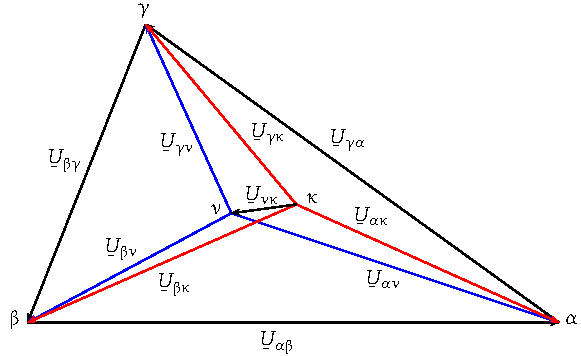
\includegraphics{Imatges/Cap-CompSim-Tensions.pdf}
\caption{Components sim\`{e}triques. Tensions fase--fase i fase--neutre}
\label{pic:Comp_sim_tens}
\end{figure}

Atenent a l'equaci\'{o} \eqref{eq:c_sim_c2}, es veu que el sistema
format per les tensions fase--fase no t\'{e} component homopolar, ja que
la seva suma  \'{e}s sempre igual a zero: $\cmplx{U}_{\alphaup\betaup} +
\cmplx{U}_{\betaup\gammaup} + \cmplx{U}_{\gammaup\alphaup} = 0$. Si a m\'{e}s
d'aquesta consideraci\'{o}, tenim en compte el que s'ha dit en l'apartat
anterior, resulta que un sistema trif\`{a}sic desequilibrat sense
neutre, es pot estudiar tenint en compte tan sols un sistema directe
i un sistema invers, ja que tant les tensions fase--fase com els
corrents de fase, no tenen component homopolar.

Pel que fa a les components directa i inversa del sistema format per
les tensions fase--fase, es compleix el seg\"{u}ent: les components
directa i inversa del sistema de tensions fase--fase, s\'{o}n
respectivament, els vectors fase--fase de les components directa i
inversa del sistema de tensions fase--neutre.

Expressant-ho en forma matem\`{a}tica tenim:
\begin{subequations}
\begin{align}
   \cmplx{U}_{\alphaup\betaup}\ap{(0)} &= 0 &
   \cmplx{U}_{\betaup\gammaup}\ap{(0)} &= 0 &
   \cmplx{U}_{\gammaup\alphaup}\ap{(0)} &= 0 \\
   \cmplx{U}_{\alphaup\betaup}\ap{(1)} &= (1-\au^2) \cmplx{U}_{\alphaup\nuup}\ap{(1)} =
   \cmplx{U}_{\alphaup\nuup}\ap{(1)} \sqrt{3}_{\measuredangle 30\degree} &
   \cmplx{U}_{\betaup\gammaup}\ap{(1)} &= \au^2 \cmplx{U}_{\alphaup\betaup}\ap{(1)} &
   \cmplx{U}_{\gammaup\alphaup}\ap{(1)} &= \au \cmplx{U}_{\alphaup\betaup}\ap{(1)} \label{eq:c_sim_a3} \\
   \cmplx{U}_{\alphaup\betaup}\ap{(2)} &= (1-\au) \cmplx{U}_{\alphaup\nuup}\ap{(2)}  =
   \cmplx{U}_{\alphaup\nuup}\ap{(2)} \sqrt{3}_{\measuredangle -30\degree}&
   \cmplx{U}_{\betaup\gammaup}\ap{(2)} &= \au \cmplx{U}_{\alphaup\betaup}\ap{(2)} &
   \cmplx{U}_{\gammaup\alphaup}\ap{(2)} &= \au^2 \cmplx{U}_{\alphaup\betaup}\ap{(2)} \label{eq:c_sim_b3}
\end{align}
\end{subequations}

En aquestes equacions s'han utilitzat les components directa i
inversa del sistema de tensions
$\cmplx{U}_{\alphaup\nuup}$, $\cmplx{U}_{\betaup\nuup}$ i $\cmplx{U}_{\gammaup\nuup}$,
per\`{o} tamb\'{e} es podrien haver utilitzat les components directa i
inversa del sistema de tensions
$\cmplx{U}_{\alphaup\kappaup}$, $\cmplx{U}_{\betaup\kappaup}$ i $\cmplx{U}_{\gammaup\kappaup}$,
ja que es compleix el seg\"{u}ent: tots el sistemes de tensi\'{o}
fase--neutre que tinguin els mateixos extrems $\alphaup, \betaup,
\gammaup$, tenen les mateixes components directa i inversa; en termes
m\'{e}s electrot\`{e}cnics, es pot dir que qualsevol joc d'imped\`{a}ncies en
estrella connectat a les mateixes fases $\alphaup, \betaup, \gammaup$,
origina unes tensions fase--neutre, les components directa i inversa
de les quals, s\'{o}n independents de les caracter\'{\i}stiques de les
imped\`{a}ncies.

El sistema de tensions fase--neutre
$\cmplx{U}_{\alphaup\nuup}$, $\cmplx{U}_{\betaup\nuup}$ i $\cmplx{U}_{\gammaup\nuup}$,
el punt neutre $\nuup$ del qual coincideix amb el baricentre del
triangle $\alphaup, \betaup,
 \gammaup$, \'{e}s l'\'{u}nic que t\'{e} un sistema homopolar nul; la resta de sistemes de tensions
 fase--neutre, com ara el format per les tensions $\cmplx{U}_{\alphaup\kappaup}$, $\cmplx{U}_{\betaup\kappaup}$ i $\cmplx{U}_{\gammaup\kappaup}$,
 el punt neutre $\kappaup$ del qual est\`{a} despla\c{c}at respecte del punt $\nuup$, tenen un sistema
 homopolar de valor:
\begin{equation}
    \cmplx{U}_{\alphaup\kappaup}\ap{(0)} = \cmplx{U}_{\betaup\kappaup}\ap{(0)} =
    \cmplx{U}_{\gammaup\kappaup}\ap{(0)} = \cmplx{U}_{\nuup\kappaup}
\end{equation}

Amb relaci\'{o} al par\`{a}graf anterior, es pot afirmar que si es
connecten tres imped\`{a}ncies id\`{e}ntiques en estrella a un sistema
de tensions trif\`{a}sic, la tensi\'{o} del punt neutre de l'estrella
coincidir\`{a} amb el baricentre $\nuup$ del triangle format per les tensions
fase--fase d'aquest sistema de tensions, i per tant les tensions fase--neutre no tindran
component homopolar; de fet, $\nuup$ \'{e}s el punt neutre de les tensions
fase--fase del sistema de tensions trif\`{a}sic.

\section{Pot\`{e}ncia} \index{pot\`{e}ncia complexa!trif\`{a}sica}

Tal com es veu en l'equaci\'{o} \eqref{eq:s_3f}, la qual fa refer\`{e}ncia a
la Figura \vref{pic:pot_comp_trif}, la pot\`{e}ncia complexa trif\`{a}sica
en un sistema desequilibrat $\cmplx{S}\ped{3F}$, es calcula a partir
de les tres tensions fase--neutre $\cmplx{U}_{\alphaup\nuup}$,
$\cmplx{U}_{\betaup\nuup}$ i $\cmplx{U}_{\gammaup\nuup}$, i dels tres
corrents de fase $\cmplx{I}_\alphaup$, $\cmplx{I}_\betaup$ i
$\cmplx{I}_\gammaup$.


No obstant, si calculem els sistemes directe, invers i homopolar,
corresponents a les tensions i corrents anteriors,
$\cmplx{U}_{\alphaup\nuup}\ap{(1)}$, $\cmplx{U}_{\alphaup\nuup}\ap{(2)}$ i
$\cmplx{U}_{\alphaup\nuup}\ap{(0)}$, i $\cmplx{I}_\alphaup\ap{(1)}$,
$\cmplx{I}_\alphaup\ap{(2)}$ i $\cmplx{I}_\alphaup\ap{(0)}$, podem
expressar la pot\`{e}ncia complexa trif\`{a}sica a partir d'aquests nous
valors, utilitzant les equacions \eqref{eq:c_sim_a},
\eqref{eq:c_sim_b} i \eqref{eq:c_sim_c}:
\begin{equation}
\begin{split}
   \cmplx{S}\ped{3F} &= \cmplx{U}_{\alphaup\nuup} \cmplx{I}_\alphaup^* +
   \cmplx{U}_{\betaup\nuup} \cmplx{I}_\betaup^* +  \cmplx{U}_{\gammaup\nuup} \cmplx{I}_\gammaup^* = \\[1ex]
   &= \big(\cmplx{U}_{\alphaup\nuup}^{(0)} + \cmplx{U}_{\alphaup\nuup}^{(1)} +
   \cmplx{U}_{\alphaup\nuup}^{(2)}\big) \big(\cmplx{I}_\alphaup^{(0)} + \cmplx{I}_\alphaup^{(1)} +
   \cmplx{I}_\alphaup^{(2)}\big)^* +  \\[1ex]
   &+ \big(\cmplx{U}_{\alphaup\nuup}^{(0)} + \au^2 \cmplx{U}_{\alphaup\nuup}^{(1)} +
   \au \cmplx{U}_{\alphaup\nuup}^{(2)} \big) \big(\cmplx{I}_\alphaup^{(0)} + \au^2 \cmplx{I}_\alphaup^{(1)}
    + \au \cmplx{I}_\alphaup^{(2)} \big)^* + \\[1ex]
   &+ \big(\cmplx{U}_{\alphaup\nuup}^{(0)} + \au \cmplx{U}_{\alphaup\nuup}^{(1)} + \au^2
   \cmplx{U}_{\alphaup\nuup}^{(2)} \big) \big(\cmplx{I}_\alphaup^{(0)} + \au
   \cmplx{I}_\alphaup^{(1)} + \au^2 \cmplx{I}_\alphaup^{(2)} \big)^* =  \\[1ex]
   &= 3\, \cmplx{U}_{\alphaup\nuup}^{(1)}  \cmplx{I}_\alphaup^{(1)*} +
   3\, \cmplx{U}_{\alphaup\nuup}^{(2)}  \cmplx{I}_\alphaup^{(2)*} +
   3\, \cmplx{U}_{\alphaup\nuup}^{(0)}  \cmplx{I}_\alphaup^{(0)*} \label{eq:c_sim_s}
\end{split}
\end{equation}

\begin{exemple}
Es tracta de trobar la pot\`{e}ncia consumida per una c\`{a}rrega trif\`{a}sica
formada per tres resist\`{e}ncies id\`{e}ntiques de $10{,}58\unit{\ohm}$,
connectades en estrella a un sistema trif\`{a}sic sense neutre, i la
tensi\'{o} a qu\`{e} est\`{a} sotmesa cada resist\`{e}ncia; els valors de les
tensions del sistema trif\`{a}sic s\'{o}n: $|\cmplx{U}_{\alphaup\betaup}| =
1840\unit{V}, |\cmplx{U}_{\betaup\gammaup}| = 2760\unit{V},
|\cmplx{U}_{\gammaup\alphaup}| = 2300\unit{V}$.

Assignem de forma arbitr\`{a}ria, tal com s'ha fet en la Figura
\vref{pic:Comp_sim_tens}, un angle de fase igual a zero, a la tensi\'{o}
$\cmplx{U}_{\alphaup\betaup}$.

A continuaci\'{o} trobem els angles $\varphi_\alphaup$ i $\varphi_\betaup$,
corresponents als v\`{e}rtexs  $\alphaup$ i $\betaup$ del triangle de
tensions, utilitzant la llei dels cosinus (vegeu la Secci\'{o}
\vref{sec:llei-s-c-t}): \index{llei dels cosinus}
\begin{align*}
    \varphi_\alphaup &= \arccos \frac{|\cmplx{U}_{\alphaup\betaup}|^2 + |\cmplx{U}_{\gammaup\alphaup}|^2 -
    |\cmplx{U}_{\betaup\gammaup}|^2}{2 |\cmplx{U}_{\alphaup\betaup}| |\cmplx{U}_{\gammaup\alphaup}|} =
    \arccos \frac{(1840\unit{V})^2 + (2300\unit{V})^2 - (2760\unit{V})^2}{2 \cdot 1840\unit{V}
    \cdot 2300\unit{V}} = 82{,}82\degree \\[1ex]
    \varphi_\betaup &= \arccos \frac{|\cmplx{U}_{\betaup\gammaup}|^2 + |\cmplx{U}_{\alphaup\betaup}|^2 -
    |\cmplx{U}_{\gammaup\alphaup}|^2}{2 |\cmplx{U}_{\betaup\gammaup}| |\cmplx{U}_{\alphaup\betaup}|} =
    \arccos \frac{(2760\unit{V})^2 + (1840\unit{V})^2 - (2300\unit{V})^2}{2 \cdot 2760\unit{V}
    \cdot 1840\unit{V}} = 55{,}77\degree
\end{align*}

Les tres tensions en forma complexa s\'{o}n doncs:
\begin{align*}
\cmplx{U}_{\alphaup\betaup} &= 1840_{\measuredangle 0\degree}\unit{V} \\
\cmplx{U}_{\betaup\gammaup} &= 2760_{\measuredangle 180\degree +
55{,}77\degree}\unit{V} =
2760_{\measuredangle 235{,}77\degree}\unit{V} \\
\cmplx{U}_{\gammaup\alphaup} &= 2300_{\measuredangle 180\degree -
82{,}82\degree}\unit{V} = 2300_{\measuredangle 97{,}18\degree}
\unit{V}
\end{align*}

Tal com s'ha dit anteriorment, el sistema de tensions fase--fase no
t\'{e} component homopolar; a m\'{e}s, el sistema de tensions fase--neutre
tampoc no en tindr\`{a}, ja que la c\`{a}rrega trif\`{a}sica \'{e}s equilibrada
(tres resist\`{e}ncies id\`{e}ntiques).

Trobem a continuaci\'{o} les components directa i inversa de les
tensions $\cmplx{U}_{\alphaup\betaup}$, $\cmplx{U}_{\betaup\gammaup}$ i
$\cmplx{U}_{\gammaup\alphaup}$, utilitzant les equacions
\eqref{eq:c_sim_a2} i \eqref{eq:c_sim_b2}:
\begin{align*}
\cmplx{U}_{\alphaup\betaup}\ap{(1)} &= \frac{1}{3} \big(
1840_{\measuredangle 0\degree}\unit{V} + 1_{\measuredangle
120\degree} \cdot 2760_{\measuredangle 235{,}77\degree}\unit{V} +
1_{\measuredangle 240\degree} \cdot 2300_{\measuredangle
97{,}18\degree}\unit{V} \big) = 2267{,}09_{\measuredangle -9{,}27\degree}\unit{V} \\[1ex]
\cmplx{U}_{\alphaup\betaup}\ap{(2)} &= \frac{1}{3} \big(
1840_{\measuredangle 0\degree}\unit{V} + 1_{\measuredangle
240\degree} \cdot 2760_{\measuredangle 235{,}77\degree}\unit{V} +
1_{\measuredangle 120\degree} \cdot 2300_{\measuredangle
97{,}18\degree}\unit{V} \big) = 539{,}77_{\measuredangle
137{,}42\degree}\unit{V} \\[1ex]
\cmplx{U}_{\alphaup\betaup}\ap{(0)} &= 0\unit{V}
\end{align*}

El seg\"{u}ent pas consisteix a trobar les components directa i inversa
de les tensions fase--neutre, utilitzant les equacions
\eqref{eq:c_sim_a3} i \eqref{eq:c_sim_b3}:
\begin{align*}
\cmplx{U}_{\alphaup\nuup}\ap{(1)} &=
\frac{\cmplx{U}_{\alphaup\betaup}\ap{(1)}}{\sqrt{3}_{\measuredangle
30\degree}} = \frac{2267{,}09_{\measuredangle
-9{,}27\degree}\unit{V}}{\sqrt{3}_{\measuredangle
30\degree}} = 1308{,}91_{\measuredangle -39{,}27\degree}\unit{V} \\[1ex]
\cmplx{U}_{\alphaup\nuup}\ap{(2)} &=
\frac{\cmplx{U}_{\alphaup\betaup}\ap{(2)}}{\sqrt{3}_{\measuredangle
-30\degree}} = \frac{539{,}77_{\measuredangle
137{,}42\degree}\unit{V}}{\sqrt{3}_{\measuredangle -30\degree}} =
311{,}64_{\measuredangle 167{,}42\degree}\unit{V} \\[1ex]
\cmplx{U}_{\alphaup\nuup}\ap{(0)} &= 0\unit{V}
\end{align*}

A partir d'aquests valors, podem calcular ara les components
directa, inversa i homopolar del corrent que circula per les
resist\`{e}ncies, aplicant les lleis de Kirchhoff; les components
directa, inversa i homopolar de les resist\`{e}ncies $R^{(1)}$,
$R^{(2)}$ i $R^{(0)}$ s\'{o}n iguals als seus valors nominals.
\begin{align*}
\cmplx{I}_\alphaup\ap{(1)} &=
\frac{\cmplx{U}_{\alphaup\nuup}\ap{(1)}}{R^{(1)}} =
\frac{1308{,}91_{\measuredangle
-39{,}27\degree}\unit{V}}{10{,}58_{\measuredangle 0 \degree}
\unit{\ohm}} =
123{,}72_{\measuredangle -39{,}27\degree}\unit{A} \\[1ex]
\cmplx{I}_\alphaup\ap{(2)} &=
\frac{\cmplx{U}_{\alphaup\nuup}\ap{(2)}}{R^{(2)}} =
\frac{311{,}64_{\measuredangle
167{,}42\degree}\unit{V}}{10{,}58_{\measuredangle 0 \degree}
\unit{\ohm}} = 29{,}46_{\measuredangle 167{,}42\degree}\unit{A} \\[1ex]
\cmplx{I}_\alphaup\ap{(0)} &=
\frac{\cmplx{U}_{\alphaup\nuup}\ap{(0)}}{R^{(0)}} =
\frac{0\unit{V}}{10{,}58_{\measuredangle 0 \degree}\unit{\ohm}} =
0\unit{A}
\end{align*}

Podem ara ja calcular la pot\`{e}ncia consumida per la c\`{a}rrega
trif\`{a}sica, utilitzant l'equaci\'{o} \eqref{eq:c_sim_s}:
\[
\begin{split}
\cmplx{S}\ped{3F} &=  3\, \cmplx{U}_{\alphaup\nuup}^{(1)}
\cmplx{I}_\alphaup^{(1)*} + 3\, \cmplx{U}_{\alphaup\nuup}^{(2)}
\cmplx{I}_\alphaup^{(2)*} +  3\,
\cmplx{U}_{\alphaup\nuup}^{(0)}  \cmplx{I}_\alphaup^{(0)*} = \\
&= 3 \cdot 1308{,}91_{\measuredangle -39{,}27\degree}\unit{V} \cdot
123{,}72_{\measuredangle 39{,}27\degree}\unit{A} + 3 \cdot
311{,}64_{\measuredangle
167{,}42\degree}\unit{V} \cdot 29{,}46_{\measuredangle -167{,}42\degree}\unit{A} + 0 = \\
&= 513{,33}\unit{kW}
\end{split}
\]

Finalment, utilitzarem les equacions \eqref{eq:c_sim_a},
\eqref{eq:c_sim_b} i \eqref{eq:c_sim_c} per trobar la tensi\'{o} a qu\`{e}
estan sotmeses les tres resist\`{e}ncies:
\begin{align*}
    \cmplx{U}_{\alphaup\nuup} &= 0 + 1308{,}91_{\measuredangle -39{,}27\degree}\unit{V} +
    311{,}64_{\measuredangle 167{,}42\degree}\unit{V}  =
    1039{,}94_{\measuredangle -47{,}01\degree}\unit{V} \\[1ex]
    \cmplx{U}_{\betaup\nuup} &= 0 + 1_{\measuredangle 240\degree} \cdot
    1308{,}91_{\measuredangle -39{,}27\degree}\unit{V} +
    1_{\measuredangle 120\degree} \cdot
    311{,}64_{\measuredangle 167{,}42\degree}\unit{V}  =
    1362{,}89_{\measuredangle -146{,}07\degree}\unit{V}    \\[1ex]
    \cmplx{U}_{\gammaup\nuup} &= 0 + 1_{\measuredangle 120\degree} \cdot
    1308{,}91_{\measuredangle -39{,}27\degree}\unit{V} +
    1_{\measuredangle 240\degree} \cdot 311{,}64_{\measuredangle 167{,}42\degree}\unit{V}  =
    1578{,}66_{\measuredangle 74{,}51\degree}\unit{V}
\end{align*}
\end{exemple}
